%% figures/fig4_harvest_lever.tex
%% Fig.4 — CPU 슬랙 하베스팅 lever 비교 (1-run Δ%, 1컬럼)

\begin{figure}[t]
\centering
\resizebox{0.95\columnwidth}{!}{%
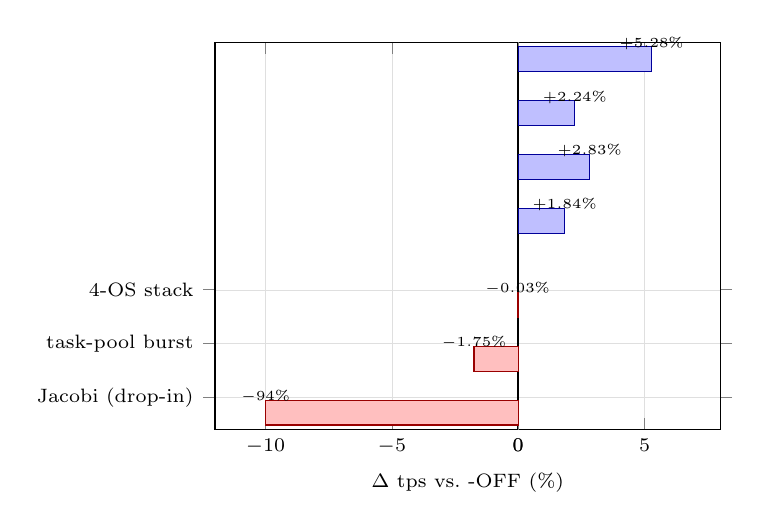
\begin{tikzpicture}
\begin{axis}[
    xbar,
    bar width=9pt,
    width=8cm, height=6.5cm,
    xlabel={$\Delta$ tps vs.\ \algname-OFF (\%)},
    xlabel style={font=\scriptsize},
    symbolic y coords={
        {Jacobi (drop-in)},
        {task-pool burst},
        {4-OS stack},
        {softmax 100ms},
        {NUMA + softmax},
        {NUMA pin},
        {branchy 100ms}},
    ytick=data,
    yticklabel style={font=\scriptsize},
    xticklabel style={font=\scriptsize},
    xmin=-12, xmax=8,
    xtick={-10,-5,0,5},
    nodes near coords,
    nodes near coords align=horizontal,
    nodes near coords style={font=\tiny},
    grid=major,
    grid style={line width=0.1pt, draw=gray!25},
    extra x ticks={0},
    extra x tick style={grid=major, grid style={black, thick}},
]
\addplot[
    fill=red!25, draw=red!60!black,
    point meta=explicit symbolic,
] coordinates {
    (-10,{Jacobi (drop-in)})   [{$-94\%$}]
    (-1.75,{task-pool burst})  [{$-1.75\%$}]
    (-0.03,{4-OS stack})       [{$-0.03\%$}]
};
\addplot[
    fill=blue!25, draw=blue!60!black,
    point meta=explicit symbolic,
] coordinates {
    (1.84,{softmax 100ms})     [{$+1.84\%$}]
    (2.83,{NUMA + softmax})    [{$+2.83\%$}]
    (2.24,{NUMA pin})          [{$+2.24\%$}]
    (5.28,{branchy 100ms})     [{$+5.28\%$}]
};
\end{axis}
\end{tikzpicture}%
}
\caption{CPU 슬랙 하베스팅 lever 단독 기여 ($\Delta$\%, \algname\ ON vs.\ OFF,
  Qwen-2.5-32B $+$ TP=4$\times$2).
  branchy $\times$ 100ms가 $+5.28\%$ (balanced cell $+12.04\%$)로 최대.
  drop-in 커널과 동일 도메인 stacking은 일관 음성. NUMA pin만 multi-run 검증 통과.}
\label{fig:harvest-lever}
\end{figure}
